\section{Motivation}

We will introduce a simple/generalized multilingual code example, discuss how
previous works perform analysis for this example, and illustrate some issue for
each approach.

Then, we introduce declarative style analysis, and show how declarative style
dataflow anlysis can be applied.

\subsection{Multilingual program}

Let's look at the following example:

Language A

public void main() \{

  Obj obj = new Obj();

  val = SOURCE;

  SINK = obj.f(val);

\}

Language B

def f(obj: Obj, param: Int): Int \{

  setField(obj, "p", param)

  val ret = getField(obj, "p")

  return ret

\}

What we are interested is whether the data stored in the node named SOURCE can
flow into the node named SINK. For example, SOURCE can be sensitive data like
smartphone's device ID (IMEI), and SINK can be an argument to a logging function.
Another example would be SOURCE being null pointer, and SINK being pointer dereference.

\subsection{Previous approaches for analyzing multilingual program}

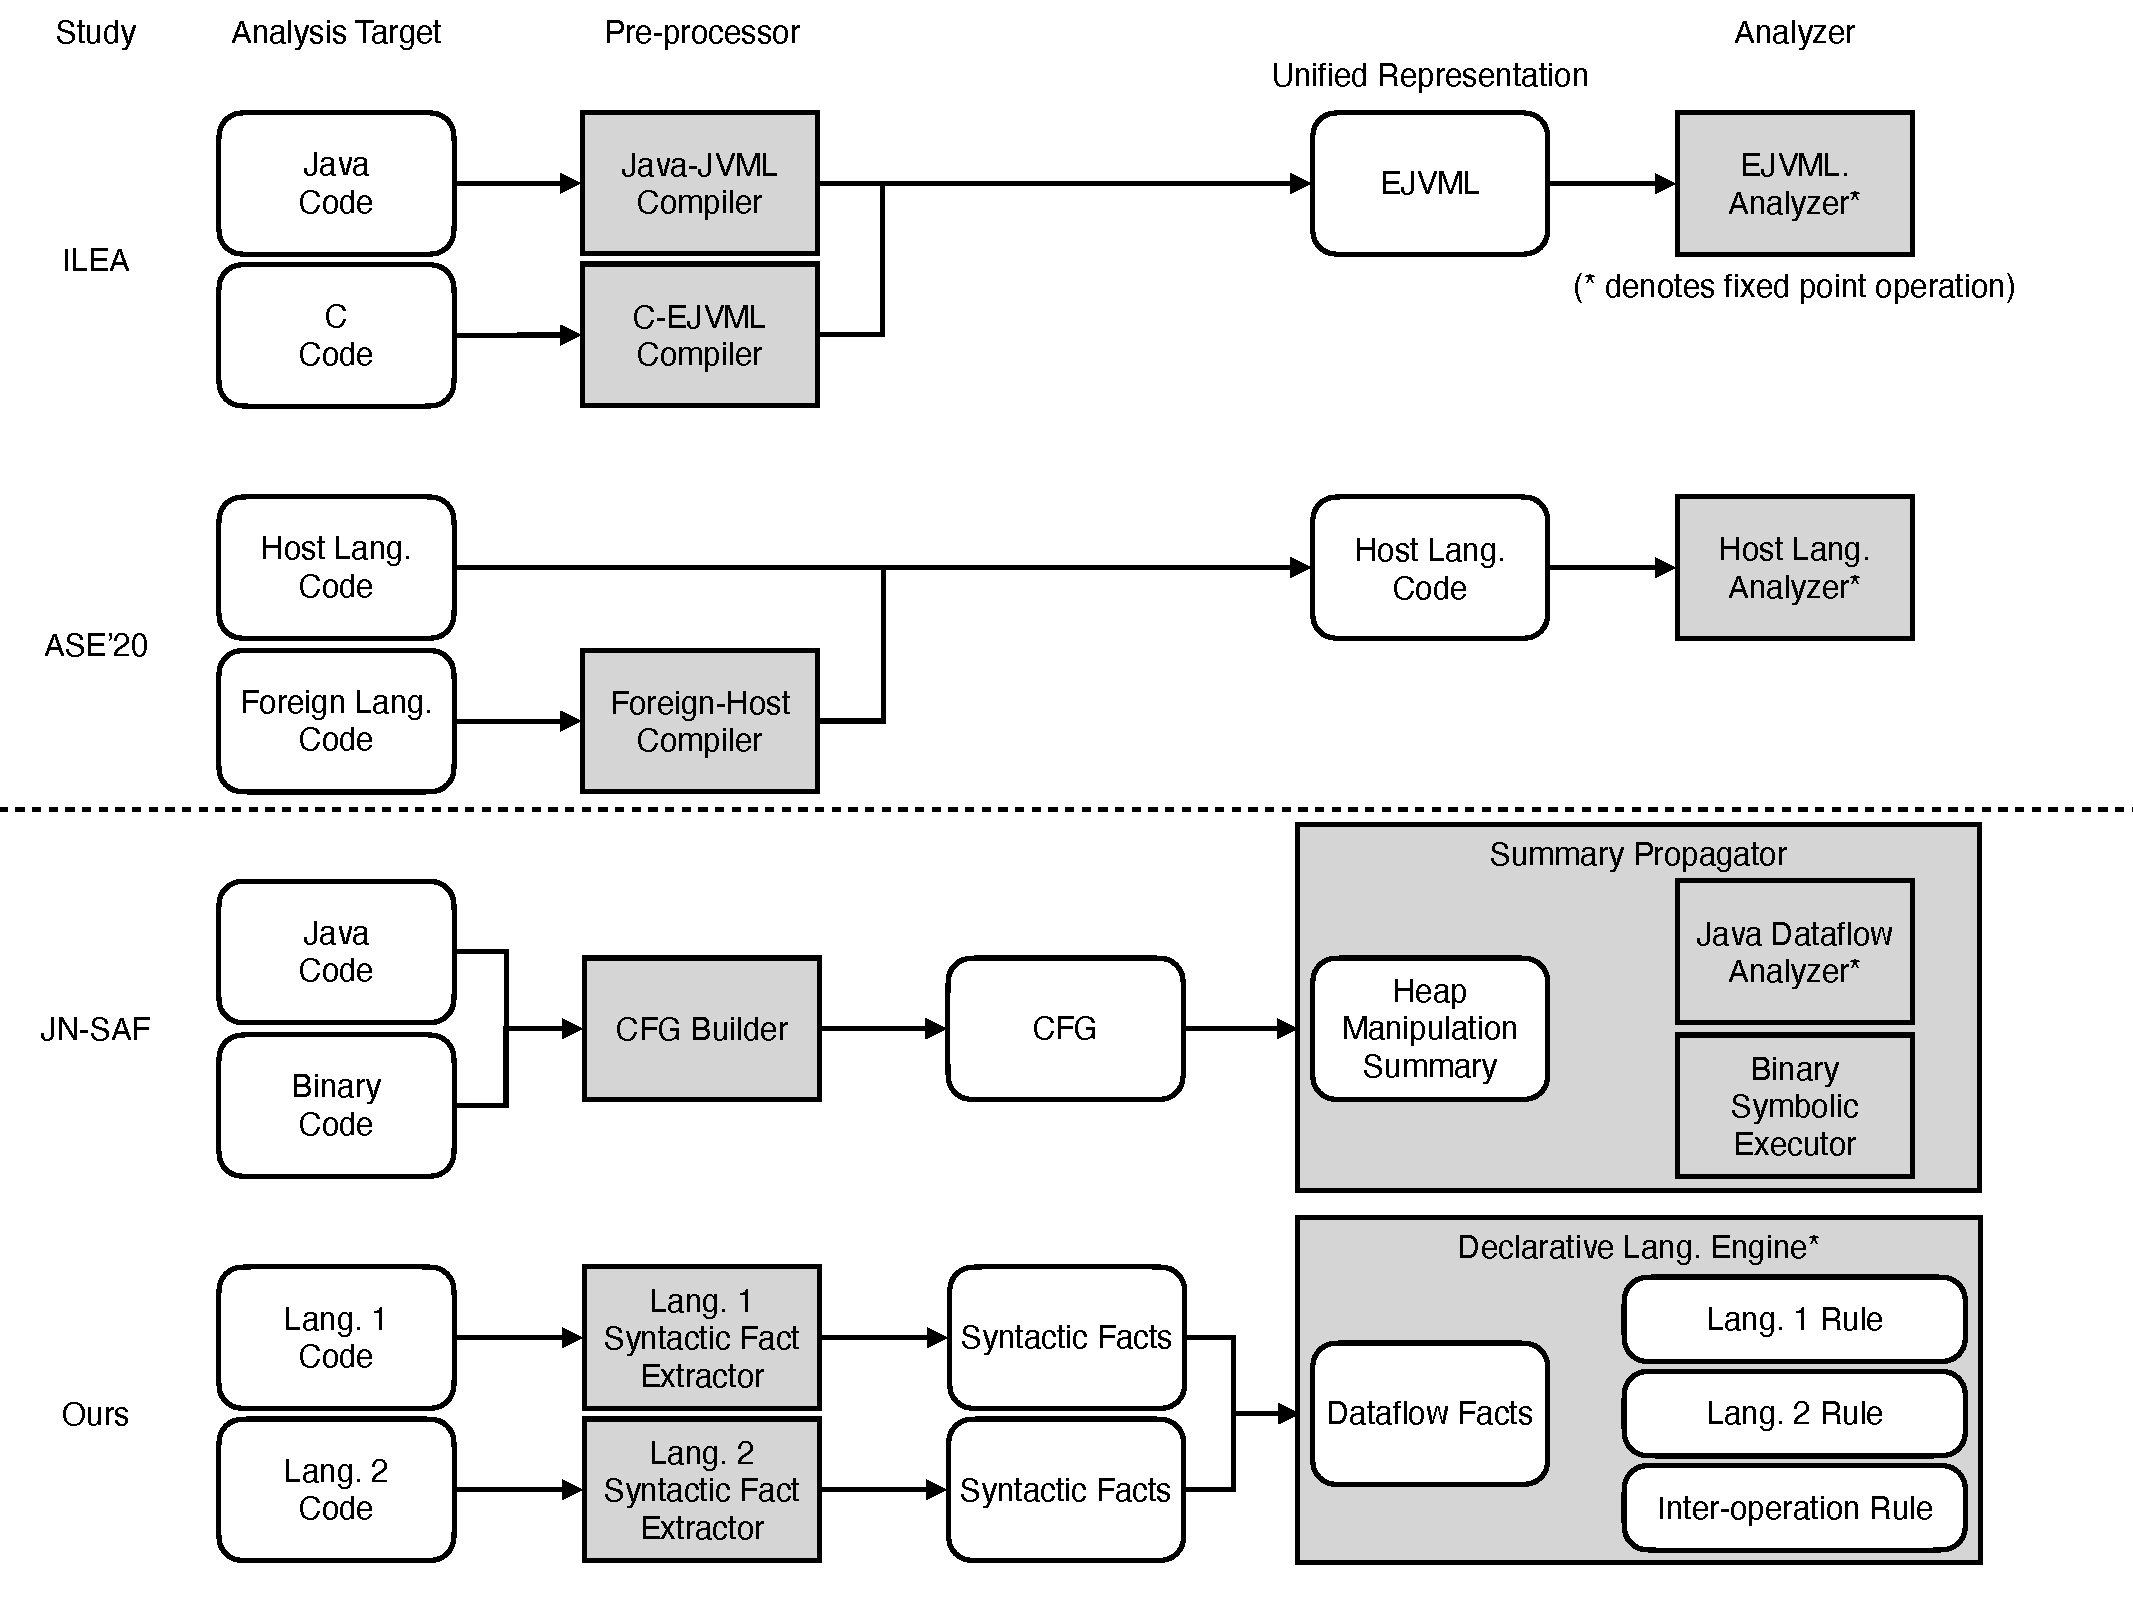
\includegraphics[width=0.5\textwidth]{img/compare}
Fig 0. Approaches for analyzing multolingual programs

There are mainly two approaces for analyzing multilingual programs. One
approach is to define host language and guest language, and transform the guest
language source code into the host language source code. The rationale behind
this approach is that one can resuse the existing analyzers for the host
language source code after the transformation is done.  ILEA[1] is a JNI
program analyzer that adopted this approach. It compiles native C code into
(extended) Java virtual machine language (EJVML), and uses existing analyzer
that works on EJVML, namely Jlint.  Recent study[2] generalizes this idea
and provides formalized method to perform analysis in more general setting.

If we apply this approach to the given example, then the function f of language
B would be compiled into language A as following:

public void f(Obj obj, int param) \{

  obj.p = param;

  int ret = obj.p;

  return ret;

\}

Then, the existing dataflow analyzer can be applied to compile code along with
original code, and would report the dataflow from SOURCE to SINK. The problem
of this approach is that ... (Compile is heavy? Challenging? Not appropriate?
Expressive power of two languaes differ and information is lost when one
language is compield to another?)

Another approach is to use a single framework which incorporates both
languages. JN-SAF[3] is a good example.  JN-SAF is a dataflow analisys tool
specialized for android applications that includes C code as binary.  The core
algorithm it uses is SBDA (summary based dataflow analysis). After constructing
call graph for both Java and native methods, "summary" for each method is
generated for each of methods. Summary is generated in bottom-up manner; if a
method calls another method, the callee method's summary is generated first and
the caller method's summary is generated, possibly using the information from
the callee's summary. (Too long?) This approach solves the problem of
comgpiling languages as previous approach, yet has some limitation in its
implementation detail.
- Symbolic execution -> heavy / slow. - Cycle in call graph -> unsound

\subsection{Declarative style analysis}

In order to solve the problem of JN-SAF, we propose the declarative style
analysis.  The biggest advantage of the declarative style analysis is that
writing analysis in declarative language is simple and light-weight, and it
does not require complex implmentation. For instance, the traditional fix-point
calucation that is used in previous approaches are handled by declarative
language engines, and the programmer for the analyzer does not need to manually
consider such semantics. All they have to write is "declaring" each rules.

For example, we can think of the rule flow(a,b) that will denote the fact that
there is a data flow from node a to node b. This rule can be defined in terms
of another preicate step:

flow(a,b):-step(a,b) or step(a,c) and flow(c,b)

where the predicate step(a,b) denotes the direct data flow from node a and b.
Given the set of facts that denote all the possible dircet steps, then all
possible flow is calculated by evaluating engine. For example, given the facts
that state

step(SOURCE, val)

step(val, param)

step(param, obj.p)

step(obj.p, ret)

step(ret, SINK)

then the declarative language engine can compute the result flow(SOURCE, SINK),
and the analyzer concludes that there is a data flow from SOURCE to SINK.

In the following sections, we formalize the general approach for performing
declartive style dataflow analysis in multilingual program (Section 3), show
the specific implementation of this appraoch for JNI programs, implemented with
CodeQL(Section 4) and show the evaluation result (Section 5).
